% Created 2025-06-10 Tue 15:17
% Intended LaTeX compiler: pdflatex
\documentclass[aspectratio=169]{beamer}
\usepackage[utf8]{inputenc}
\usepackage[T1]{fontenc}
\usepackage{graphicx}
\usepackage{longtable}
\usepackage{wrapfig}
\usepackage{rotating}
\usepackage[normalem]{ulem}
\usepackage{amsmath}
\usepackage{amssymb}
\usepackage{capt-of}
\usepackage{hyperref}
\usepackage[style=apa, backend=biber]{biblatex}
\DeclareLanguageMapping{american}{american-apa}
\addbibresource{./refs/refs.bib}
\AtEveryBibitem{\clearfield{note}}
\usepackage{endnotes}
\let\footnote=\endnote
\usepackage{./jtc}
\usetheme{default}
\author{Evan Misshula}
\date{\today}
\title{Introduction to Machine Learning: Modeling, Training and Evaluation}
\hypersetup{
 pdfauthor={Evan Misshula},
 pdftitle={Introduction to Machine Learning: Modeling, Training and Evaluation},
 pdfkeywords={},
 pdfsubject={},
 pdfcreator={Emacs 29.3 (Org mode 9.6.15)}, 
 pdflang={English}}
\begin{document}

\maketitle
g
\section{Workflow}
\label{sec:orgd6313b7}
\begin{frame}[label={sec:org3e22840}]{End to end process}
Recall \alert{ML workflow} is a sequence of steps to build and deploy a model that
solves a problem using data.
\end{frame}

\begin{frame}[label={sec:orgf2b260e}]{The pipeline}
\begin{center}
\begin{tabular}{llll}
Ingestion \& Preprocessing & Analysis & \alert{Modeling} & Deployment\\[0pt]
\hline
Definition & EDA & \alert{Selection} & Tuning\\[0pt]
Data Collection & Feature Engineering & \alert{Training} & Deployment\\[0pt]
Cleaning &  & \alert{Evaluation} & Monitoring\\[0pt]
\end{tabular}
\end{center}
\end{frame}

\begin{frame}[label={sec:org3a3b71d}]{ML Workflow Graph}
\begin{figure}[htbp]
\centering
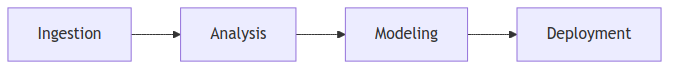
\includegraphics[width=.9\linewidth]{workflow.png}
\caption{ML workflow steps rendered as a flowchart}
\end{figure}


\begin{center}
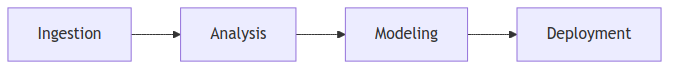
\includegraphics[width=.9\linewidth]{workflow.png}
\end{center}
\end{frame}

\section{Training}
\label{sec:org9811b6d}
\begin{frame}[label={sec:orgfcdaea7}]{What is Model Training?}
\begin{itemize}
\item Model training is the process of estimating parameters \(\theta\) of a model \(f_\theta(x)\) using data \(\{(x_i, y_i)\}_{i=1}^n\).
\item Typically achieved by minimizing a loss function:
\begin{equation}
\hat{\theta} = \arg\min_\theta \frac{1}{n} \sum_{i=1}^n \mathcal{L}(f_\theta(x_i), y_i)
\end{equation}
\item Common loss functions:
\begin{itemize}
\item \alert{\alert{Squared error loss}} (regression): \(\mathcal{L}(\hat{y}, y) = (\hat{y} - y)^2\)
\item \alert{\alert{Cross-entropy loss}} (classification):
\end{itemize}
\end{itemize}
\begin{equation}
    \mathcal{L}(\hat{y}, y) = -\sum_{c} \1_{\{y = c\}} \log \hat{p}_c
\1_{\{x = 1\}}
\end{equation}
\end{frame}


\section{Loss Functions}
\label{sec:orgcf16470}
\begin{frame}[label={sec:orgda7d3f1}]{Cross-Entropy Loss (Classification)}
The cross-entropy loss measures how well a predicted probability
distribution \(\hat{p}\) matches the true label \(y\).

For a multiclass classification problem:
\begin{equation}
\mathcal{L}(\hat{y}, y) = -\sum_{c=1}^C \mathds{1}_{\{y = c\}} \log \hat{p}_c
\end{equation}

\begin{itemize}
\item \(\hat{p}_c\): predicted probability for class \(c\)
\item \(y\): true class label
\item Only the log probability of the true class contributes to the loss.
\end{itemize}
\end{frame}

\begin{frame}[label={sec:org215a98d}]{Binary Cross-Entropy Example}
\begin{equation}
\mathcal{L}(\hat{y}, y) = -[y \log(\hat{y}) + (1 - y) \log(1 - \hat{y})]
\end{equation}
\end{frame}

\begin{frame}[label={sec:org7cea1e5}]{Interpretation}
\begin{itemize}
\item Penalizes confident wrong predictions heavily.
\item Encourages models to predict probabilities that reflect the actual distribution.
\end{itemize}
\end{frame}



\begin{frame}[label={sec:org9517556}]{Training vs Generalization}
\begin{itemize}
\item \alert{Empirical risk} (training error):
\begin{equation}
\hat{R}(\theta) = \frac{1}{n} \sum_{i=1}^n \mathcal{L}(f_\theta(x_i), y_i)
\end{equation}
\item \alert{Expected risk} (true/generalization error):
\begin{equation}
R(\theta) = \mathbb{E}_{(x,y) \sim \mathcal{D}} \left[ \mathcal{L}(f_\theta(x), y) \right]
\end{equation}
\item Generalization gap: \(R(\theta) - \hat{R}(\theta)\)
\item Overfitting: small \(\hat{R}\), large \(R\)
\end{itemize}
\end{frame}


\section{Generalization and Expected Risk}
\label{sec:org59e4aa6}
\begin{frame}[label={sec:org76a9c71}]{What Is Expected Risk?}
The \alert{expected risk} or \alert{generalization error} is the average loss over the true data distribution \(\mathcal{D}\):

\begin{equation}
R(\theta) = \mathbb{E}_{(x,y) \sim \mathcal{D}} \left[ \mathcal{L}(f_\theta(x), y) \right]
\end{equation}

\begin{itemize}
\item \(\theta\): model parameters
\item \(f_\theta(x)\): model prediction
\item \(\mathcal{L}\): loss function (e.g., squared error)
\item \(\mathcal{D}\): unknown true distribution of the data
\end{itemize}
\end{frame}

\begin{frame}[label={sec:orge3b7af3}]{Why It Matters}
\begin{itemize}
\item It tells us how well the model will perform \alert{on new data}.
\item Since \(\mathcal{D}\) is unknown, we estimate it using validation or test sets.
\end{itemize}
\end{frame}

\begin{frame}[label={sec:org8c0c23d}]{Empirical vs Expected Risk}
\begin{center}
\begin{tabular}{lll}
Risk Type & Expression & Description\\[0pt]
\hline
Empirical Risk & \(\hat{R}(\theta) = \frac{1}{n} \sum_{i=1}^{n} \mathcal{L}(f_\theta(x_i), y_i)\) & Error on training data\\[0pt]
Expected Risk & \(R(\theta) = \mathbb{E}_{(x,y) \sim \mathcal{D}} [\mathcal{L}(f_\theta(x), y)]\) & Error on all data\\[0pt]
\end{tabular}
\end{center}

\begin{itemize}
\item Goal: Minimize expected risk while avoiding overfitting.
\item Overfitting in practical terms means complicating the model so
that it lowers the Emperical Risk without lowering the Expected Risk
\end{itemize}
\end{frame}


\section{Evaluation}
\label{sec:org236ad27}
\begin{frame}[label={sec:org5328148}]{Evaluation Metrics}
\begin{itemize}
\item \alert{Regression}:
\begin{itemize}
\item Mean Squared Error (MSE): 
\[
    \text{MSE} = \frac{1}{n} \sum_{i=1}^n (\hat{y}_i - y_i)^2
    \]
\item \(R^2\) score:
\[
    R^2 = 1 - \frac{\sum_i (\hat{y}_i - y_i)^2}{\sum_i (y_i - \bar{y})^2}
    \]
\end{itemize}

\item \alert{Classification}:
\begin{itemize}
\item Accuracy: \(\text{Accuracy} = \frac{1}{n} \sum_{i=1}^n \mathds{1}_{\{\hat{y}_i = y_i\}}\)
\item Precision: \(\frac{\text{TP}}{\text{TP} + \text{FP}}\)
\item Recall: \(\frac{\text{TP}}{\text{TP} + \text{FN}}\)
\item F1 score: harmonic mean of precision and recall
\[
    F1 = 2 \cdot \frac{\text{Precision} \cdot \text{Recall}}{\text{Precision} + \text{Recall}}
    \]
\end{itemize}
\end{itemize}
\end{frame}


\begin{frame}[label={sec:org5de2fae}]{Overview of Classification Metrics}
Different tasks prioritize different types of error.

\begin{center}
\begin{tabular}{lll}
Metric & Measures & Use Case\\[0pt]
\hline
Accuracy & Overall correctness & Balanced datasets\\[0pt]
Precision & True positives among predicted pos & False positives are costly (e.g., spam)\\[0pt]
Recall & True positives among actual pos & False negatives are costly (e.g., disease)\\[0pt]
F1 Score & Harmonic mean of P and R & Imbalanced data, cost for FP and FN\\[0pt]
ROC AUC & Probabilistic ranking & Model comparison, threshold tuning\\[0pt]
\end{tabular}
\end{center}
\end{frame}

\section{Accuracy}
\label{sec:org9b1f2af}
\begin{frame}[label={sec:orgc3336b3}]{Definition and Intuition}
\[
\text{Accuracy} = \frac{TP + TN}{TP + FP + TN + FN}
\]
\begin{itemize}
\item Correct predictions / Total predictions
\item Best for balanced datasets
\end{itemize}
\end{frame}

\section{Precision and Recall}
\label{sec:org96df35a}
\begin{frame}[label={sec:org2a45f28}]{Precision}
\[
\text{Precision} = \frac{TP}{TP + FP}
\]
\begin{itemize}
\item How many predicted positives are truly positive?
\item High precision = few false positives
\end{itemize}
\end{frame}

\begin{frame}[label={sec:org2d6b18c}]{Recall}
\[
\text{Recall} = \frac{TP}{TP + FN}
\]
\begin{itemize}
\item How many actual positives were correctly predicted?
\item High recall = few false negatives
\end{itemize}
\end{frame}

\section{F1 Score}
\label{sec:org29564bc}
\begin{frame}[label={sec:orgfaf8b4d}]{Balancing Precision and Recall}
\[
F1 = 2 \cdot \frac{\text{Precision} \cdot \text{Recall}}{\text{Precision} + \text{Recall}}
\]
\begin{itemize}
\item Harmonic mean of precision and recall
\item Use when both types of error matter
\item Good for imbalanced datasets
\end{itemize}
\end{frame}

\section{ROC and AUC}
\label{sec:org4ae8d3a}
\begin{frame}[label={sec:orge28c4b9}]{Receiver Operating Characteristic}
\begin{itemize}
\item Plot of True Positive Rate vs. False Positive Rate at various thresholds
\item Area Under Curve (AUC) ranges from 0.5 (random) to 1.0 (perfect)
\end{itemize}

\[
\text{TPR} = \frac{TP}{TP + FN}, \quad \text{FPR} = \frac{FP}{FP + TN}
\]

\begin{itemize}
\item AUC is threshold-independent
\item Use when you want to compare classifiers
\end{itemize}
\end{frame}

\section{Summary of classification metrics}
\label{sec:orgee144ba}
\begin{frame}[label={sec:org36277e9}]{Choosing the Right Metric}
\begin{itemize}
\item Accuracy: for balanced classes
\item Precision: when false positives are costly
\item Recall: when false negatives are costly
\item F1: when both matter, especially in imbalanced data
\item AUC: for ranking models across thresholds
\end{itemize}
\end{frame}


\begin{frame}[label={sec:org62667be}]{Cross-Validation}
\begin{itemize}
\item Cross-validation estimates generalization error by partitioning data.
\item \alert{k-fold CV}:
\begin{itemize}
\item Split data into \(k\) disjoint subsets.
\item For each \(i = 1, \ldots, k\):
\begin{itemize}
\item Train on \(k-1\) folds
\item Evaluate on fold \(i\)
\end{itemize}
\item Average the evaluation metrics.
\end{itemize}
\end{itemize}
\end{frame}

\begin{frame}[label={sec:orgd6bff1e}]{Bias-Variance Tradeoff}
\begin{itemize}
\item Expected prediction error at point \(x\):
\[
  \mathbb{E}[(f(x) - y)^2] = \underbrace{[\mathbb{E}(f(x)) - y]^2}_{\text{Bias}^2} + \underbrace{\mathbb{E}[(f(x) - \mathbb{E}(f(x)))^2]}_{\text{Variance}} + \underbrace{\sigma^2}_{\text{Irreducible error}}
  \]
\item Simple models: low variance, high bias
\item Complex models: low bias, high variance
\end{itemize}
\end{frame}

\begin{frame}[label={sec:org0391ca9}]{Model Selection}
\begin{itemize}
\item Choose the best model using a \alert{validation set} or \alert{cross-validation}.
\item Avoid tuning hyperparameters using the test set.
\item Balance:
\begin{itemize}
\item Training error
\item Generalization performance
\item Computational cost
\end{itemize}
\end{itemize}
\end{frame}

\section{Model Selection and Tuning}
\label{sec:org356eb3d}
\begin{frame}[label={sec:org753ba95}]{Hyperparameter Tuning}
Some model settings are not learned from data but must be specified
manually — these are \alert{hyperparameters}.

\begin{center}
\begin{tabular}{ll}
Model & Hyperparameter Examples\\[0pt]
\hline
k-NN & Number of neighbors \(k\)\\[0pt]
Decision Tree & Max depth, min samples per leaf\\[0pt]
Lasso/Ridge & Regularization strength \(\alpha\)\\[0pt]
Neural Network & Learning rate, batch size\\[0pt]
\end{tabular}
\end{center}
\end{frame}

\begin{frame}[label={sec:org726f797}]{Why Tune Hyperparameters?}
\begin{itemize}
\item Improve generalization
\item Prevent overfitting
\item Optimize computational efficiency
\end{itemize}
\end{frame}

\begin{frame}[label={sec:org5fb02ad}]{Best Practices}
\begin{itemize}
\item Use a \alert{validation set} or \alert{cross-validation} to evaluate each
setting.
\item Never use the \alert{test set} for tuning — it must simulate unseen data.
\end{itemize}
\end{frame}

\begin{frame}[label={sec:org4ec5187}]{Trade-offs}
\begin{itemize}
\item Training error vs validation error
\item Model complexity vs performance
\item Runtime vs accuracy
\end{itemize}
\end{frame}

\begin{frame}[label={sec:org68bff67}]{Tools}
\begin{itemize}
\item Grid search, random search, or Bayesian optimization
\end{itemize}
\end{frame}

\begin{frame}[label={sec:orgd336f16}]{Summary Training and Evaluation}
\begin{itemize}
\item Training minimizes empirical loss.
\item Evaluation uses test or validation data.
\item Use metrics appropriate for the task.
\item Cross-validation provides robust error estimates.
\item The bias-variance tradeoff is fundamental in choosing models.
\end{itemize}
\end{frame}
\end{document}
